% Unified IR M2b + V&V — plan bundle
% Compile: pdflatex plan.tex
%
% plan.pdf is intentionally absent. The TeX waiver granted on 2026-08-28 and
% re-authorised for this phase stands: no TeX, Tectonic or Pandoc toolchain is
% installed and none may be installed. This bundle (.tex + .tikz + .mmd) is the
% reproducible source and is the deliverable. Recorded waiver, not an unmet
% §11 halt condition.

\documentclass[11pt,a4paper]{article}
\usepackage[T1]{fontenc}
\usepackage[utf8]{inputenc}
\usepackage[margin=25mm]{geometry}
\usepackage{booktabs}
\usepackage{longtable}
\usepackage{pifont}
\usepackage{tikz}
\usetikzlibrary{positioning,fit,backgrounds,arrows.meta,calc}
\usepackage{hyperref}
\hypersetup{colorlinks=true,linkcolor=blue!50!black,urlcolor=blue!50!black}
\newcommand{\code}[1]{\texttt{#1}}

\title{Unified IR --- M2b, V\&V first\\[2pt]
       \large A durable verification structure, then the first consumer migration}
\author{HyMeKo framework}
\date{Created-at: \textbf{2026-08-29 02:11 CEST}}

\begin{document}
\maketitle

\begin{abstract}
\noindent
Authorisation, quoted verbatim:
\begin{quote}\code{APPROVED-CORE-EDIT: unified-ir-m2b-vv-core-consumers}\end{quote}

\noindent
Two pieces of work, in this order and not the reverse: build a durable
verification and validation structure with a measured coverage baseline, and
only then migrate the read-only IR consumers in this repository. The ordering is
the point --- a migration measured against no baseline cannot be shown to have
preserved anything.
\end{abstract}

\section{Scope}

\paragraph{In scope.} The unified-IR V\&V structure; reorganisation of the
existing M0.5/M0.6/M2a tests; migration of \code{hymeko\_core} read-only
consumers; \emph{if and only if} the core gates pass, migration of
\code{hymeko\_hnn} read-only IR access; the documentation, benchmark and
coverage artifacts these require.

\paragraph{Out of scope.} ID representation; stable or generational arenas;
mutation or transaction APIs; lowering, construction or serde storage layout;
the canonical hash algorithm; the wire protocol; dependencies or
\code{Cargo.lock}; \code{unsafe} or \code{get\_unchecked}; sibling repositories;
the three IFAC artifacts.

\section{Estimated time}

\begin{longtable}{@{}lp{6.6cm}r@{}}
\toprule
\textbf{Stage} & \textbf{Basis} & \textbf{ETA} \\
\midrule
\endhead
Preflight + plan & state verification, document reading, this bundle & 0.5\,h \\
Coverage tool & \code{cargo-llvm-cov} install; the vendored parent config
  replaces crates.io, so the install runs from a temporary directory outside
  that tree & 0.5\,h \\
Baseline & full gate plus one instrumented run ($\approx$5\,min each) & 0.75\,h \\
V\&V restructure & \code{git mv} of 9 files, deduplication of 4 corpus walkers,
  requirements and traceability & 1.5\,h \\
Fault injection & 4 mutations, one full suite each at $\approx$72\,s & 0.75\,h \\
Core migration & 9 consumer sites plus equivalence tests & 1.0\,h \\
HNN migration & 7 sites plus derived-view equivalence & 0.75\,h \\
Coverage delta, benchmarks, report, publish & & 1.25\,h \\
\midrule
\textbf{Total} & sequential, single implementer & \textbf{$\approx$7\,h} \\
\bottomrule
\end{longtable}

\section{Affected files}

\paragraph{Tests --- moved, not copied.}
\code{unified\_ir\_m05/\{builder,oracle,invariance,depth\}.rs},
\code{unified\_ir\_m06/\{coverage,frozen\_v1,coherence\_tests\}.rs} and
\code{unified\_ir\_m2a/\{accessors,sentinel\}.rs} move by \code{git mv} into
\code{unified\_ir/\{support,verification,validation\}/}.

\paragraph{Tests --- new.} \code{support/corpus.rs} (consolidates four copies of
the same fixture walk), \code{validation/consumer\_equivalence.rs},
\code{validation/derived\_views.rs}, and focused guards added to
\code{verification/access.rs} after fault injection.

\paragraph{Production --- migrated.} \code{util/pretty\_print.rs},
\code{writers/ir\_writer.rs}, \code{hymeko\_hnn/traversal/hypergraphview.rs}.

\paragraph{Production --- deliberately not migrated.} \code{ir/ir.rs} (storage
implementation), \code{ir/lower.rs} (construction), \code{ir/canonical\_hash.rs}
and \code{ir/hash\_pass.rs} (representation-owner algorithms),
\code{ir/coherence.rs} (must read raw storage to \emph{detect} incoherence),
serde derives, and tests that construct malformed state on purpose.

\paragraph{Documentation.} \code{docs/verification/unified-ir/*},
\code{reports/2026-08-29-unified-ir-m2b-vv.md},
\code{scripts/coverage\_summary.awk}, updates to the migration, consumer-map and
dynamic-test-plan documents.

\section{Coverage definitions}

\paragraph{Denominator.} \code{cargo llvm-cov} instruments workspace members
only, so \code{tests/}, \code{benches/}, \code{examples/}, \code{target/},
\code{vendor/} and external dependencies are already absent from the report ---
verified by inspecting the emitted \code{SF:} records, not assumed. The
classifier in \code{scripts/coverage\_summary.awk} labels every record and would
make any leakage visible as a non-\code{production} category.

\paragraph{No production source is excluded.} Not one path is filtered out to
improve a number.

\paragraph{Reported separately} --- because collapsing them would mislead:
workspace production; \code{hymeko\_core/src/ir}; each touched file;
implemented-requirement coverage; and end-state requirement coverage.

\paragraph{Branch coverage is not available.} \code{cargo llvm-cov --branch} is
marked \emph{unstable} and needs a nightly toolchain; this host is stable
1.97.1. Every \code{BRF} record is therefore structurally \code{0}. The summary
prints \code{n/a} rather than \code{0\,\%}, because ``no branch data'' and ``no
branches covered'' are different claims. \textbf{No estimate is substituted.}

\paragraph{Skips during profile collection.} Two, both by command line, neither
in source:
\begin{itemize}\itemsep2pt
  \item \code{test\_load\_meta\_geometry} --- the known 57/58 drift, which
        continues to run and fail unchanged in the normal gate;
  \item \code{test\_coo\_construction\_throughput} --- a \emph{timed} assertion.
        Coverage instrumentation adds counters to every branch, so a throughput
        threshold is not merely slower but meaningless. It passes in the
        uninstrumented gate.
\end{itemize}

\section{Test strategy}

\begin{description}\itemsep3pt
\item[Verification] Boundary and negative cases for every accessor: \code{NONE},
  exact end, end+1, far out of range, across all four id types; mapping absent,
  present, present-but-record-missing, present-but-back-link-wrong; root, leaf,
  single child, multiple siblings; iterator id/record pairing and exact
  cardinality; \code{U1} slot order; malformed-state coherence findings.
\item[Validation] The 96-fixture corpus; before/after consumer equivalence
  against a reference walk that still indexes storage directly; derived
  \code{HyperGraphView} incidence coverage.
\item[Test strength] Four injected defects, each required to be caught by a
  \emph{named} test. Mutated production code is never committed, and restoration
  is proved by hash.
\item[Not written] No dummy tests for the dynamic API. Add/remove, stale ids,
  cascade policy, transaction rollback, batch atomicity, snapshot isolation and
  distributed replay are recorded as \code{PLANNED}/\code{BLOCKED} against M3/M4.
  A test asserting the shape of something unimplemented inflates the count and
  the coverage while establishing nothing.
\end{description}

\section{Performance budget}

The accessor microbenchmarks are \emph{not} re-run as a campaign:
\code{ir/access.rs} is byte-identical to its M2a.1 state, so the M2a.1 verdicts
(\code{SCALAR ZERO-COST}, \code{SCAN WITHIN-NOISE}, \code{MAP WITHIN-NOISE},
\code{CHECKED-COMPOSITE equivalent}) carry forward. Only cells whose inputs
actually changed are measured: \code{HyperGraphView::from\_ir} construction and
the end-to-end read traversal. Gate: $<3\,\%$ regression, quiet host,
alternating variants.

\section{Rollback}

Three independent commits. The V\&V baseline commit touches no production source
and can stand alone. The core migration touches two files. The HNN migration
touches one. Any of the three reverts without the others.

\section{Risk anticipation}

\paragraph{The mechanical-substitution trap.} \code{node\_for\_decl} is
\emph{not} a drop-in for \code{decl\_to\_node[d.0]}: it additionally resolves the
record and validates its back-link, which is more work and different behaviour
on malformed input. The HNN edge scan contains exactly such a map-only read, and
a search-and-replace migration would have silently changed it.

\paragraph{Coverage as false comfort.} Both migrated core consumers had
\textbf{0\,\%} baseline coverage --- the edits landed in code nothing checked. A
coverage number alone would not have revealed that; reading the per-file report
before editing did.

\paragraph{Worst-case input.} The corpus is 96 fixtures, 6\,840 declarations,
maximum depth 5. That is the real production scale; nothing here is measured
only at toy size.

\section{Figures}

% Unified IR M2b + V&V — figures (TikZ)
% Created-at: 2026-08-29 02:11 CEST
% APPROVED-CORE-EDIT: unified-ir-m2b-vv-core-consumers
% % Unified IR M2b + V&V — figures (TikZ)
% Created-at: 2026-08-29 02:11 CEST
% APPROVED-CORE-EDIT: unified-ir-m2b-vv-core-consumers
% % Unified IR M2b + V&V — figures (TikZ)
% Created-at: 2026-08-29 02:11 CEST
% APPROVED-CORE-EDIT: unified-ir-m2b-vv-core-consumers
% \input{plan.tikz} from plan.tex, which supplies the preamble.

% ---------------------------------------------------------------------------
% Figure 1 — the V&V split, and why it is not decorative.
% ---------------------------------------------------------------------------
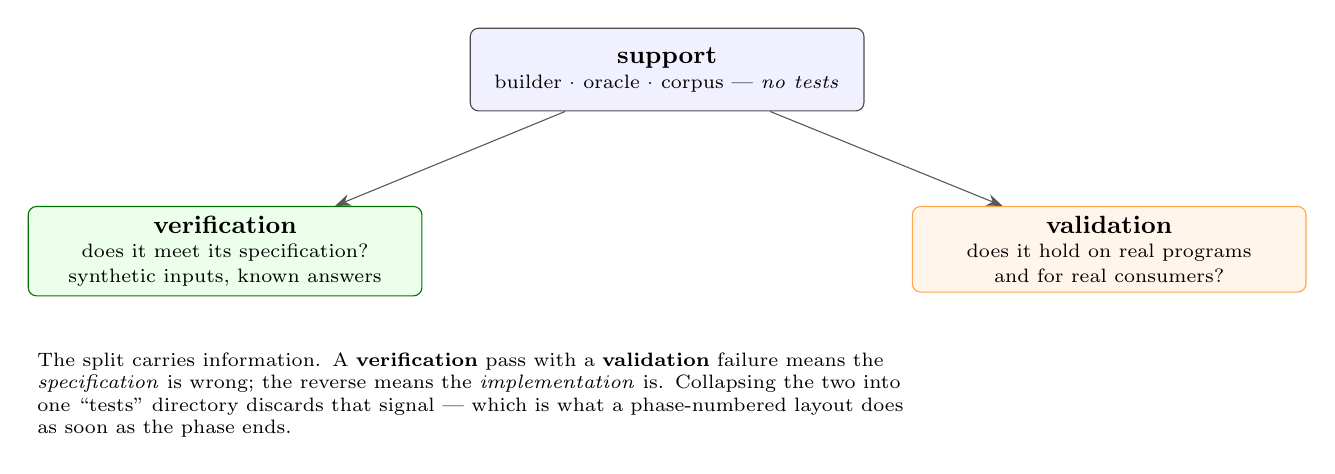
\begin{tikzpicture}[
    font=\small,
    lay/.style={draw=black!70, rounded corners=3pt, minimum width=5.0cm,
                minimum height=1.05cm, align=center},
    sup/.style={lay, fill=blue!6},
    ver/.style={lay, fill=green!8, draw=green!45!black},
    val/.style={lay, fill=orange!8, draw=orange!70},
    a/.style={-{Stealth[length=2mm]}, black!65},
    node distance=0.55cm and 2.0cm,
]
\node[sup] (s) {\textbf{support}\\[-2pt]\scriptsize builder · oracle · corpus --- \emph{no tests}};
\node[ver, below left=1.2cm and 0.6cm of s] (v)
      {\textbf{verification}\\[-2pt]\scriptsize does it meet its specification?\\[-2pt]\scriptsize synthetic inputs, known answers};
\node[val, below right=1.2cm and 0.6cm of s] (a)
      {\textbf{validation}\\[-2pt]\scriptsize does it hold on real programs\\[-2pt]\scriptsize and for real consumers?};
\draw[a] (s) -- (v);
\draw[a] (s) -- (a);

\node[align=left, anchor=north west, font=\scriptsize, text width=11.2cm]
      at ($(v.south west)+(0,-0.6)$)
      {The split carries information. A \textbf{verification} pass with a
       \textbf{validation} failure means the \emph{specification} is wrong; the
       reverse means the \emph{implementation} is. Collapsing the two into one
       ``tests'' directory discards that signal --- which is what a
       phase-numbered layout does as soon as the phase ends.};
\end{tikzpicture}

% ---------------------------------------------------------------------------
% Figure 2 — what coverage does not tell you.
%
% All four mutants were planted in code that line coverage already reported as
% executed. Coverage located none of them.
% ---------------------------------------------------------------------------
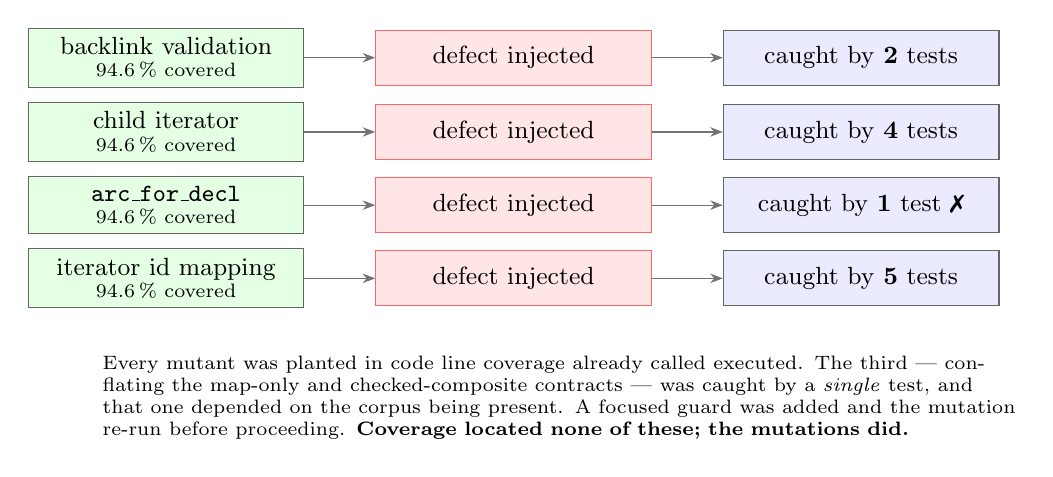
\begin{tikzpicture}[
    font=\small,
    cell/.style={draw=black!60, minimum width=3.5cm, minimum height=0.7cm, align=center},
    covd/.style={cell, fill=green!10},
    mut/.style={cell, fill=red!10, draw=red!60},
    cau/.style={cell, fill=blue!8},
    node distance=0.18cm and 0.9cm,
]
\node[covd] (c1) {backlink validation\\[-3pt]\scriptsize 94.6\,\% covered};
\node[covd, below=of c1] (c2) {child iterator\\[-3pt]\scriptsize 94.6\,\% covered};
\node[covd, below=of c2] (c3) {\code{arc\_for\_decl}\\[-3pt]\scriptsize 94.6\,\% covered};
\node[covd, below=of c3] (c4) {iterator id mapping\\[-3pt]\scriptsize 94.6\,\% covered};

\node[mut, right=of c1] (m1) {defect injected};
\node[mut, right=of c2] (m2) {defect injected};
\node[mut, right=of c3] (m3) {defect injected};
\node[mut, right=of c4] (m4) {defect injected};

\node[cau, right=of m1] (k1) {caught by \textbf{2} tests};
\node[cau, right=of m2] (k2) {caught by \textbf{4} tests};
\node[cau, right=of m3] (k3) {caught by \textbf{1} test \ding{55}};
\node[cau, right=of m4] (k4) {caught by \textbf{5} tests};

\foreach \i in {1,2,3,4} {
  \draw[-{Stealth[length=1.6mm]}, black!55] (c\i) -- (m\i);
  \draw[-{Stealth[length=1.6mm]}, black!55] (m\i) -- (k\i);
}

\node[align=left, anchor=north west, font=\scriptsize, text width=11.6cm]
      at ($(k4.south west)+(-8.0,-0.5)$)
      {Every mutant was planted in code line coverage already called executed.
       The third --- conflating the map-only and checked-composite contracts ---
       was caught by a \emph{single} test, and that one depended on the corpus
       being present. A focused guard was added and the mutation re-run before
       proceeding. \textbf{Coverage located none of these; the mutations did.}};
\end{tikzpicture}
 from plan.tex, which supplies the preamble.

% ---------------------------------------------------------------------------
% Figure 1 — the V&V split, and why it is not decorative.
% ---------------------------------------------------------------------------
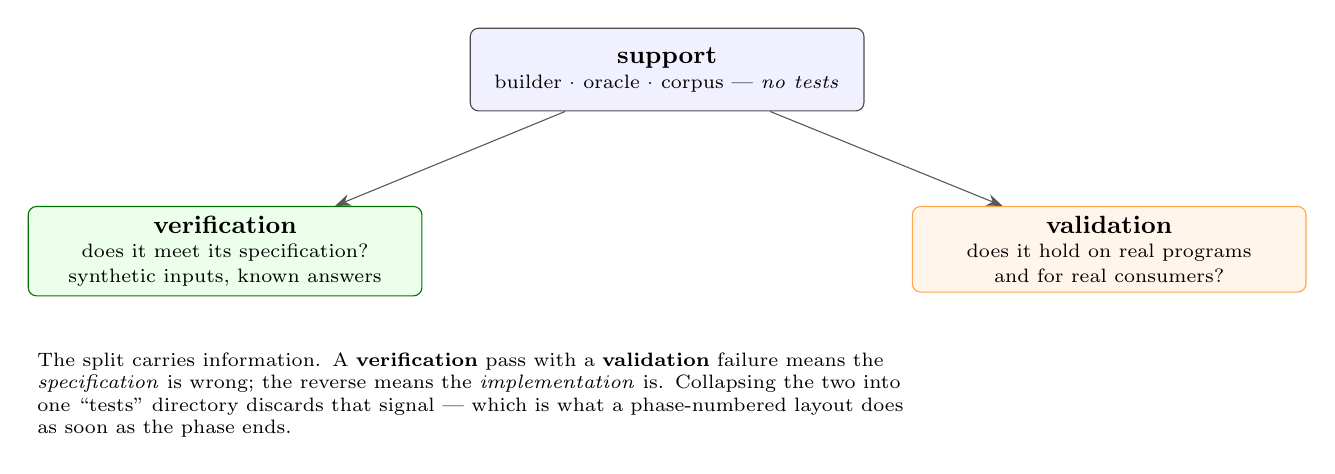
\begin{tikzpicture}[
    font=\small,
    lay/.style={draw=black!70, rounded corners=3pt, minimum width=5.0cm,
                minimum height=1.05cm, align=center},
    sup/.style={lay, fill=blue!6},
    ver/.style={lay, fill=green!8, draw=green!45!black},
    val/.style={lay, fill=orange!8, draw=orange!70},
    a/.style={-{Stealth[length=2mm]}, black!65},
    node distance=0.55cm and 2.0cm,
]
\node[sup] (s) {\textbf{support}\\[-2pt]\scriptsize builder · oracle · corpus --- \emph{no tests}};
\node[ver, below left=1.2cm and 0.6cm of s] (v)
      {\textbf{verification}\\[-2pt]\scriptsize does it meet its specification?\\[-2pt]\scriptsize synthetic inputs, known answers};
\node[val, below right=1.2cm and 0.6cm of s] (a)
      {\textbf{validation}\\[-2pt]\scriptsize does it hold on real programs\\[-2pt]\scriptsize and for real consumers?};
\draw[a] (s) -- (v);
\draw[a] (s) -- (a);

\node[align=left, anchor=north west, font=\scriptsize, text width=11.2cm]
      at ($(v.south west)+(0,-0.6)$)
      {The split carries information. A \textbf{verification} pass with a
       \textbf{validation} failure means the \emph{specification} is wrong; the
       reverse means the \emph{implementation} is. Collapsing the two into one
       ``tests'' directory discards that signal --- which is what a
       phase-numbered layout does as soon as the phase ends.};
\end{tikzpicture}

% ---------------------------------------------------------------------------
% Figure 2 — what coverage does not tell you.
%
% All four mutants were planted in code that line coverage already reported as
% executed. Coverage located none of them.
% ---------------------------------------------------------------------------
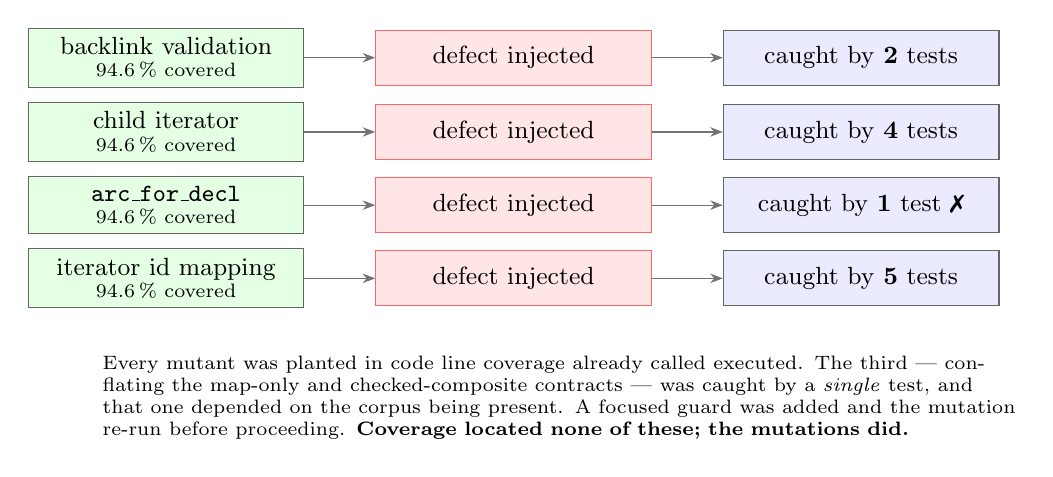
\begin{tikzpicture}[
    font=\small,
    cell/.style={draw=black!60, minimum width=3.5cm, minimum height=0.7cm, align=center},
    covd/.style={cell, fill=green!10},
    mut/.style={cell, fill=red!10, draw=red!60},
    cau/.style={cell, fill=blue!8},
    node distance=0.18cm and 0.9cm,
]
\node[covd] (c1) {backlink validation\\[-3pt]\scriptsize 94.6\,\% covered};
\node[covd, below=of c1] (c2) {child iterator\\[-3pt]\scriptsize 94.6\,\% covered};
\node[covd, below=of c2] (c3) {\code{arc\_for\_decl}\\[-3pt]\scriptsize 94.6\,\% covered};
\node[covd, below=of c3] (c4) {iterator id mapping\\[-3pt]\scriptsize 94.6\,\% covered};

\node[mut, right=of c1] (m1) {defect injected};
\node[mut, right=of c2] (m2) {defect injected};
\node[mut, right=of c3] (m3) {defect injected};
\node[mut, right=of c4] (m4) {defect injected};

\node[cau, right=of m1] (k1) {caught by \textbf{2} tests};
\node[cau, right=of m2] (k2) {caught by \textbf{4} tests};
\node[cau, right=of m3] (k3) {caught by \textbf{1} test \ding{55}};
\node[cau, right=of m4] (k4) {caught by \textbf{5} tests};

\foreach \i in {1,2,3,4} {
  \draw[-{Stealth[length=1.6mm]}, black!55] (c\i) -- (m\i);
  \draw[-{Stealth[length=1.6mm]}, black!55] (m\i) -- (k\i);
}

\node[align=left, anchor=north west, font=\scriptsize, text width=11.6cm]
      at ($(k4.south west)+(-8.0,-0.5)$)
      {Every mutant was planted in code line coverage already called executed.
       The third --- conflating the map-only and checked-composite contracts ---
       was caught by a \emph{single} test, and that one depended on the corpus
       being present. A focused guard was added and the mutation re-run before
       proceeding. \textbf{Coverage located none of these; the mutations did.}};
\end{tikzpicture}
 from plan.tex, which supplies the preamble.

% ---------------------------------------------------------------------------
% Figure 1 — the V&V split, and why it is not decorative.
% ---------------------------------------------------------------------------
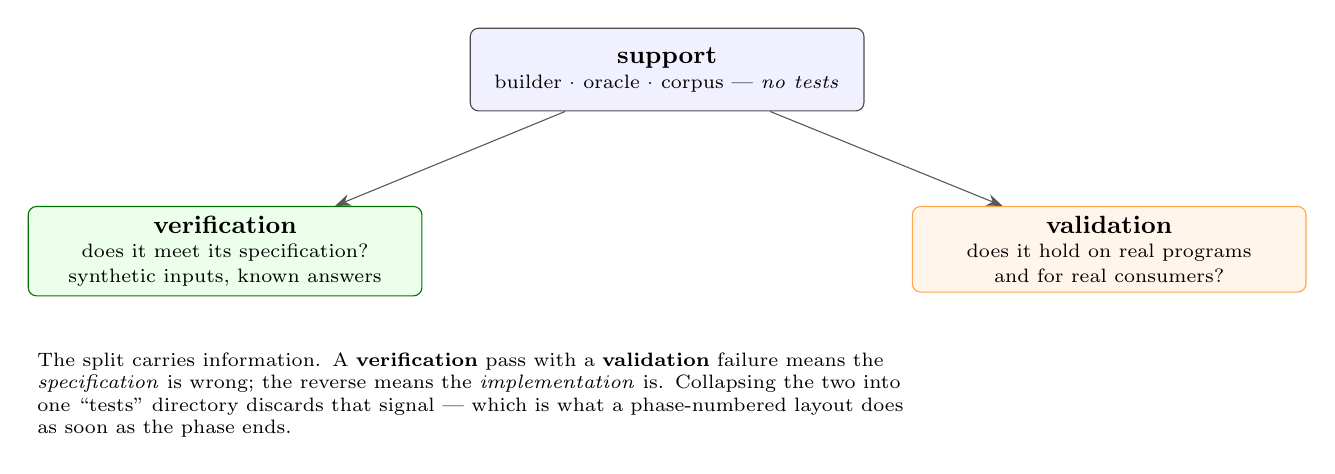
\begin{tikzpicture}[
    font=\small,
    lay/.style={draw=black!70, rounded corners=3pt, minimum width=5.0cm,
                minimum height=1.05cm, align=center},
    sup/.style={lay, fill=blue!6},
    ver/.style={lay, fill=green!8, draw=green!45!black},
    val/.style={lay, fill=orange!8, draw=orange!70},
    a/.style={-{Stealth[length=2mm]}, black!65},
    node distance=0.55cm and 2.0cm,
]
\node[sup] (s) {\textbf{support}\\[-2pt]\scriptsize builder · oracle · corpus --- \emph{no tests}};
\node[ver, below left=1.2cm and 0.6cm of s] (v)
      {\textbf{verification}\\[-2pt]\scriptsize does it meet its specification?\\[-2pt]\scriptsize synthetic inputs, known answers};
\node[val, below right=1.2cm and 0.6cm of s] (a)
      {\textbf{validation}\\[-2pt]\scriptsize does it hold on real programs\\[-2pt]\scriptsize and for real consumers?};
\draw[a] (s) -- (v);
\draw[a] (s) -- (a);

\node[align=left, anchor=north west, font=\scriptsize, text width=11.2cm]
      at ($(v.south west)+(0,-0.6)$)
      {The split carries information. A \textbf{verification} pass with a
       \textbf{validation} failure means the \emph{specification} is wrong; the
       reverse means the \emph{implementation} is. Collapsing the two into one
       ``tests'' directory discards that signal --- which is what a
       phase-numbered layout does as soon as the phase ends.};
\end{tikzpicture}

% ---------------------------------------------------------------------------
% Figure 2 — what coverage does not tell you.
%
% All four mutants were planted in code that line coverage already reported as
% executed. Coverage located none of them.
% ---------------------------------------------------------------------------
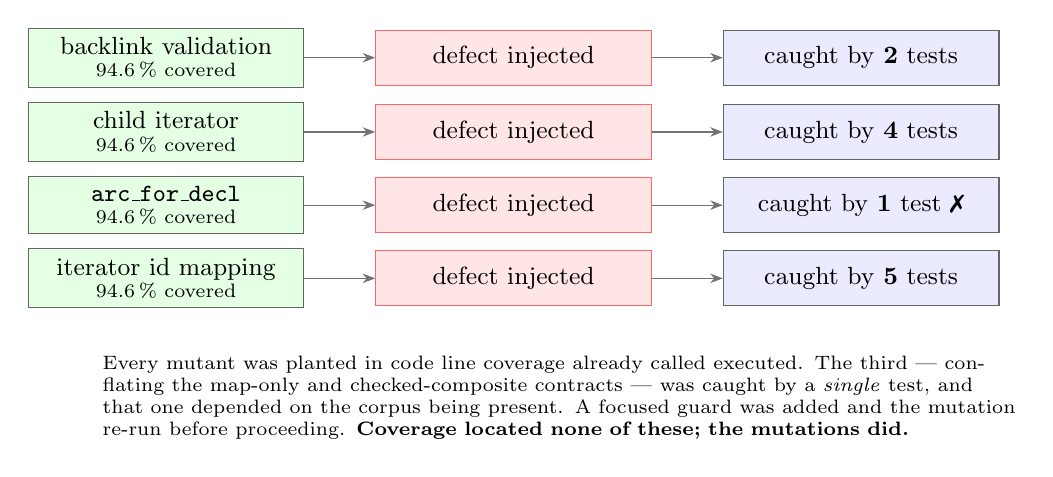
\begin{tikzpicture}[
    font=\small,
    cell/.style={draw=black!60, minimum width=3.5cm, minimum height=0.7cm, align=center},
    covd/.style={cell, fill=green!10},
    mut/.style={cell, fill=red!10, draw=red!60},
    cau/.style={cell, fill=blue!8},
    node distance=0.18cm and 0.9cm,
]
\node[covd] (c1) {backlink validation\\[-3pt]\scriptsize 94.6\,\% covered};
\node[covd, below=of c1] (c2) {child iterator\\[-3pt]\scriptsize 94.6\,\% covered};
\node[covd, below=of c2] (c3) {\code{arc\_for\_decl}\\[-3pt]\scriptsize 94.6\,\% covered};
\node[covd, below=of c3] (c4) {iterator id mapping\\[-3pt]\scriptsize 94.6\,\% covered};

\node[mut, right=of c1] (m1) {defect injected};
\node[mut, right=of c2] (m2) {defect injected};
\node[mut, right=of c3] (m3) {defect injected};
\node[mut, right=of c4] (m4) {defect injected};

\node[cau, right=of m1] (k1) {caught by \textbf{2} tests};
\node[cau, right=of m2] (k2) {caught by \textbf{4} tests};
\node[cau, right=of m3] (k3) {caught by \textbf{1} test \ding{55}};
\node[cau, right=of m4] (k4) {caught by \textbf{5} tests};

\foreach \i in {1,2,3,4} {
  \draw[-{Stealth[length=1.6mm]}, black!55] (c\i) -- (m\i);
  \draw[-{Stealth[length=1.6mm]}, black!55] (m\i) -- (k\i);
}

\node[align=left, anchor=north west, font=\scriptsize, text width=11.6cm]
      at ($(k4.south west)+(-8.0,-0.5)$)
      {Every mutant was planted in code line coverage already called executed.
       The third --- conflating the map-only and checked-composite contracts ---
       was caught by a \emph{single} test, and that one depended on the corpus
       being present. A focused guard was added and the mutation re-run before
       proceeding. \textbf{Coverage located none of these; the mutations did.}};
\end{tikzpicture}


\noindent
Restructure, migration-eligibility and gate-sequence views are in
\code{plan.mmd}.

\end{document}
